\documentclass[twocolumn]{article}

% \usepackage{eclbkbox}
% \usepackage{amsmath}
% \usepackage{amssymb}
% \usepackage{amscd}
% \usepackage{xy}
\usepackage{graphicx}
% \usepackage{fancyhdr}
% \usepackage{color}
% \usepackage[dark,all,bottom,landscape,timestamp]{draftcopy}
% \usepackage{everypage}

% \usepackage{ulem}
% go back to italics for emphasis, though
% \normalem


% \AddEverypageHook{\waterb}

% \fancyhead[LE,RO]{\slshape page number}
% \fancyhead[RE]{\slshape \LaTeX}
% \fancyhead[LO]{\slshape \LaTeX}
% \fancyfoot[LO,LE]{\slshape ! LaTeX Error: Something's wrong---perhaps a missing $\backslash$item?}
% \fancyfoot[C]{}
% \fancyfoot[RO,RE]{\slshape $\heartsuit\hspace{-1.5em}\longrightarrow$ }

% \draftcopyName{DRAFT!}{300}
% \pagestyle{fancy}

\begin{document} 

\title{ {\bf You Keep Dying } }
\author{Tom~Murphy~VII}
\date{1 April 2010}

\maketitle

\begin{abstract}
We present a new programming language called Wikiplia. The language
has an unprecedented level of integration: The system is its own
compiler, language definition, documentation, development environment,
distributed filesystem, database, revision control system,
bootstrapping software license, community message board, and World
Wide Web home site. Wikiplia is designed to be Free to a greater
extent and in more dimensions than existing languages.
\end{abstract}

\footnotetext[-1]{Copyright \copyright\ 2010 the Regents of the Wikiplia
Foundation. Appears in SIGBOVIK 2010 with the permission of the
Association for Computational Heresy; {\em IEEEEEE!} press,
Verlag-Verlag volume no.~0x40-2A.
\pounds 0.00}

\vspace{1em}
{\noindent \small {\bf Keywords}:
  Freedom, programming language, software license, wiki, XML, 
  weatherproof footwear and their fastening mechanisms,
  hyper-driven devices
}

% copyright notice generated automatically from Year and author.
% permission added if \permission{} given.


\section{Introduction}


\begin{figure}[t]
\begin{center}
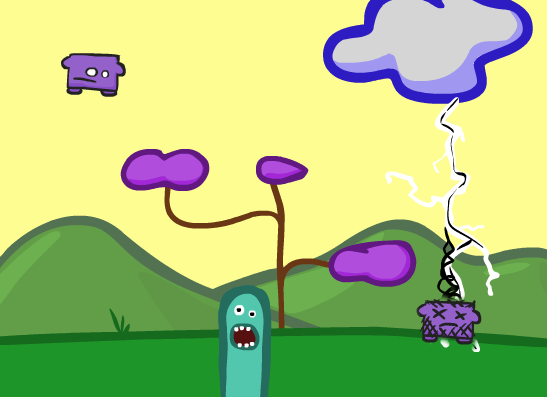
\includegraphics[width=0.43\textwidth]{lightning}
\end{center}
\caption{You keep conduct the lightning\ \ and\ \ you keep dying} \label{fig:lightning}
\end{figure}

NetCraft confirms it. *LF is dying.
I believe children are our future or futures.

\end{document}
